\documentclass[tikz,border=10pt]{standalone}
\usepackage{helvet}
\renewcommand{\familydefault}{\sfdefault}
\usepackage{tikz}
\usepackage{amsmath}
\usetikzlibrary{calc, positioning, arrows.meta, fit, shapes.geometric, decorations.pathreplacing}

\definecolor{emeraldpine}{HTML}{1A4D3E}
\definecolor{harvardcrimson}{HTML}{A51C30}
\definecolor{ethdarkblue}{HTML}{1F407A}
\definecolor{ethpetrol}{HTML}{007A87}
\definecolor{ethbronze}{HTML}{B87333}
\definecolor{ink}{HTML}{1A202C}
\definecolor{cardbg}{HTML}{F8FAFC}
\definecolor{shadecolor}{HTML}{F4F6F9}
\definecolor{paleink}{HTML}{A0AEC0}

\begin{document}
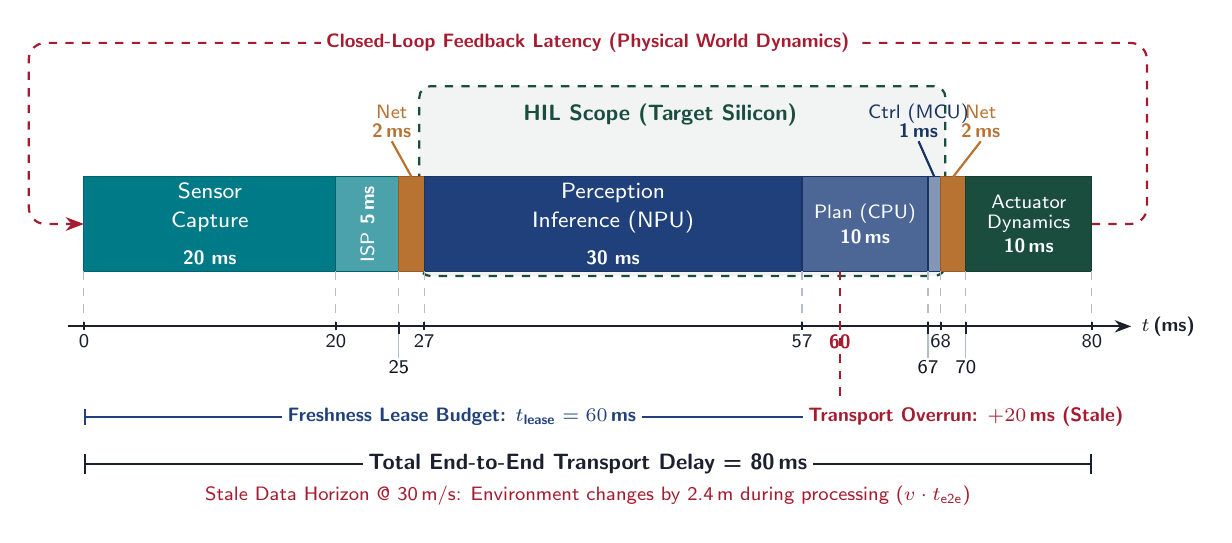
\begin{tikzpicture}[
    font=\sffamily,
    arr/.style={-{Stealth[scale=1.2]}, thick, ink},
    looparr/.style={-{Stealth[scale=1.0]}, thick, dashed, harvardcrimson}
]

% Scaling factor: 1 ms = 0.16 cm. Total = 80 ms = 12.8 cm.
\def\scale{0.16}
\def\h{1.2} % height of pipeline blocks

% Coordinates for the start of each block
\coordinate (x0) at (0, 0);
\coordinate (x1) at ($(x0) + (20*\scale, 0)$);
\coordinate (x2) at ($(x1) + (5*\scale, 0)$);
\coordinate (x3) at ($(x2) + (2*\scale, 0)$);
\coordinate (x4) at ($(x3) + (30*\scale, 0)$);
\coordinate (x_lease) at ($(x0) + (60*\scale, 0)$);
\coordinate (x5) at ($(x4) + (10*\scale, 0)$);
\coordinate (x6) at ($(x5) + (1*\scale, 0)$);
\coordinate (x7) at ($(x6) + (2*\scale, 0)$);
\coordinate (x8) at ($(x7) + (10*\scale, 0)$);

% HIL Scope Box (Target Silicon / Device Under Test)
% Encloses Perception (x3) to Control (x6)
\draw[thick, dashed, emeraldpine, fill=emeraldpine!6!white, rounded corners=4pt] 
    ($(x3) + (-0.06, -0.06)$) rectangle ($(x6) + (0.06, \h+1.15)$);
\node[emeraldpine, font=\footnotesize\bfseries, anchor=north] 
    at ($ (x3)!0.5!(x5) + (-0.2, \h+1.05) $) {HIL Scope (Target Silicon)};

% 1. Sensor Capture (20 ms) = 3.2 cm
\draw[fill=ethpetrol, draw=ethpetrol!80!black] (x0) rectangle ++(20*\scale, \h) 
    node[midway, white, align=center] {\footnotesize Sensor\\[-0.3ex] \footnotesize Capture\\[0.3ex] \scriptsize \textbf{20 ms}};

% 2. ISP (5 ms) = 0.8 cm
\draw[fill=ethpetrol!70!white, draw=ethpetrol!80!black] (x1) rectangle ++(5*\scale, \h) 
    node[midway, white, rotate=90, font=\scriptsize] {ISP \textbf{5\,ms}};

% 3. Net1 (2 ms) = 0.32 cm
\coordinate (net1_top) at ($(x2) + (1.0*\scale, \h)$);
\draw[fill=ethbronze, draw=ethbronze!80!black] (x2) rectangle ++(2*\scale, \h);
\draw[ethbronze, thick] (net1_top) -- ($(net1_top) + (-0.25, 0.45)$);
\node[above, text=ethbronze, font=\scriptsize, align=center, inner sep=1pt] 
    at ($(net1_top) + (-0.25, 0.45)$) {Net\\[-0.3ex] \textbf{2\,ms}};

% 4. Perception (30 ms) = 4.8 cm
\draw[fill=ethdarkblue, draw=ethdarkblue!80!black] (x3) rectangle ++(30*\scale, \h) 
    node[midway, white, align=center] {\footnotesize Perception\\[-0.3ex] \footnotesize Inference (NPU)\\[0.3ex] \scriptsize \textbf{30 ms}};

% 5. Planning (10 ms) = 1.6 cm
\draw[fill=ethdarkblue!80!white, draw=ethdarkblue!80!black] (x4) rectangle ++(10*\scale, \h) 
    node[midway, white, align=center, font=\scriptsize] {Plan (CPU)\\[0.3ex] \textbf{10\,ms}};

% 6. Control (1 ms) = 0.16 cm
\coordinate (ctrl_top) at ($(x5) + (0.5*\scale, \h)$);
\draw[fill=ethdarkblue!55!white, draw=ethdarkblue!80!black] (x5) rectangle ++(1*\scale, \h);
\draw[ethdarkblue!80!black, thick] (ctrl_top) -- ($(ctrl_top) + (-0.20, 0.45)$);
\node[above, text=ethdarkblue!80!black, font=\scriptsize, align=center, inner sep=1pt] 
    at ($(ctrl_top) + (-0.20, 0.45)$) {Ctrl (MCU)\\[-0.3ex] \textbf{1\,ms}};

% 7. Net2 (2 ms) = 0.32 cm
\coordinate (net2_top) at ($(x6) + (1.0*\scale, \h)$);
\draw[fill=ethbronze, draw=ethbronze!80!black] (x6) rectangle ++(2*\scale, \h);
\draw[ethbronze, thick] (net2_top) -- ($(net2_top) + (0.35, 0.45)$);
\node[above, text=ethbronze, font=\scriptsize, align=center, inner sep=1pt] 
    at ($(net2_top) + (0.35, 0.45)$) {Net\\[-0.3ex] \textbf{2\,ms}};

% 8. Actuator (10 ms) = 1.6 cm
\draw[fill=emeraldpine, draw=emeraldpine!80!black] (x7) rectangle ++(10*\scale, \h) 
    node[midway, white, align=center, font=\scriptsize] {Actuator\\[-0.3ex] \scriptsize Dynamics\\[0.3ex] \scriptsize \textbf{10\,ms}};

% Feedback Loop (Orthogonal routing around the pipeline)
\draw[looparr, rounded corners=6pt] 
    ($(x8) + (0, \h/2)$) -- ++(0.7, 0) -- ++(0, 2.3) -- ++(-80*\scale-1.4, 0) -- ++(0, -2.3) -- (x0 |- 0, \h/2);
\node[fill=white, text=harvardcrimson, font=\scriptsize\bfseries, inner sep=2pt] 
    at ($ (x0)!0.5!(x8) + (0, \h/2 + 2.3) $) {Closed-Loop Feedback Latency (Physical World Dynamics)};

% Vertical drop lines from stage boundaries to timeline axis
\foreach \pt in {x0, x1, x2, x3, x4, x5, x6, x7, x8} {
    \draw[paleink!80!white, thin, dashed] (\pt) -- ++(0, -0.68);
}

% Freshness Lease Vertical Line (60 ms) from pipeline bottom to bracket
\draw[thick, dashed, harvardcrimson] (x_lease) -- ++(0, -1.95);

% Timeline Axis at y = -0.70
\coordinate (tl_start) at (0, -0.70);
\coordinate (tl_end) at ($(80*\scale, -0.70)$);
\draw[thick, ink, -{Stealth[scale=0.9]}] ($(tl_start) + (-0.2, 0)$) -- ($(tl_end) + (0.5, 0)$) 
    node[right, font=\scriptsize\bfseries, text=ink] {$t$\,(ms)};

% Cumulative Ticks
% Level 1 ticks (y = -0.70 to -0.95): 0, 20, 27, 57, 68, 80 ms
\foreach \xval/\lbl in {0/0, 20/20, 27/27, 57/57, 68/68, 80/80} {
    \draw[thick, ink] (\xval*\scale, -0.65) -- (\xval*\scale, -0.75);
    \node[below, font=\scriptsize, text=ink, inner sep=1pt] at (\xval*\scale, -0.77) {\lbl};
}

% 60 ms tick on axis (highlighted in crimson)
\draw[thick, harvardcrimson] (60*\scale, -0.65) -- (60*\scale, -0.75);
\node[below, font=\scriptsize\bfseries, text=harvardcrimson, inner sep=1pt] at (60*\scale, -0.77) {60};

% Level 2 ticks (staggered below for tight regions): 25, 67, 70 ms
\foreach \xval/\lbl in {25/25, 67/67, 70/70} {
    \draw[thick, ink] (\xval*\scale, -0.65) -- (\xval*\scale, -0.80);
    \draw[paleink!80!white, thin] (\xval*\scale, -0.80) -- (\xval*\scale, -1.10);
    \node[below, font=\scriptsize, text=ink!70!black, inner sep=1pt] at (\xval*\scale, -1.10) {\lbl};
}

% Freshness Lease Bracket (0 to 60 ms)
\coordinate (fl_start) at (0, -1.85);
\coordinate (fl_end) at (60*\scale, -1.85);
\draw[{Bar[width=2mm]}-{Bar[width=2mm]}, thick, ethdarkblue] (fl_start) -- (fl_end) 
    node[midway, fill=white, font=\scriptsize\bfseries, text=ethdarkblue, inner sep=2pt] 
    {Freshness Lease Budget: $t_{\text{lease}} = 60$\,ms};

% Lease Breach Segment (60 to 80 ms)
\draw[{Bar[width=2mm]}-{Bar[width=2mm]}, thick, harvardcrimson] (60*\scale, -1.85) -- (80*\scale, -1.85)
    node[midway, fill=white, font=\scriptsize\bfseries, text=harvardcrimson, inner sep=2pt] 
    {Transport Overrun: $+20$\,ms (Stale)};

% Total End-to-End Transport Delay Bar
\coordinate (c_start) at (0, -2.45);
\coordinate (c_end) at (80*\scale, -2.45);
\draw[{Bar[width=2.5mm]}-{Bar[width=2.5mm]}, thick, ink] (c_start) -- (c_end) 
    node[midway, fill=white, font=\footnotesize\bfseries, text=ink, inner sep=2pt] 
    {Total End-to-End Transport Delay = 80\,ms};

% Stale Data Horizon
\node[anchor=north, font=\scriptsize, text=harvardcrimson, align=center] 
    at ($ (c_start)!0.5!(c_end) + (0, -0.15) $) 
    {Stale Data Horizon @ 30\,m/s: Environment changes by 2.4\,m during processing ($v \cdot t_{\text{e2e}}$)};

\end{tikzpicture}
\end{document}
